\section{Web-based demo system}
In order to better illustrate the work that have been done in this final year project, a web-based demo system was also implemented based on Django, which is a popular Python web framework. For the back end, Django connected previous python modules like extracting SIFT features and calculating EMD distance. For the front end, a CSS library called Bootstrap was used for better visualization. Also, ajax was heavily used to connect the user input with the back end server and dynamically update the web page. \\

\begin{figure}[!ht]
\centering
	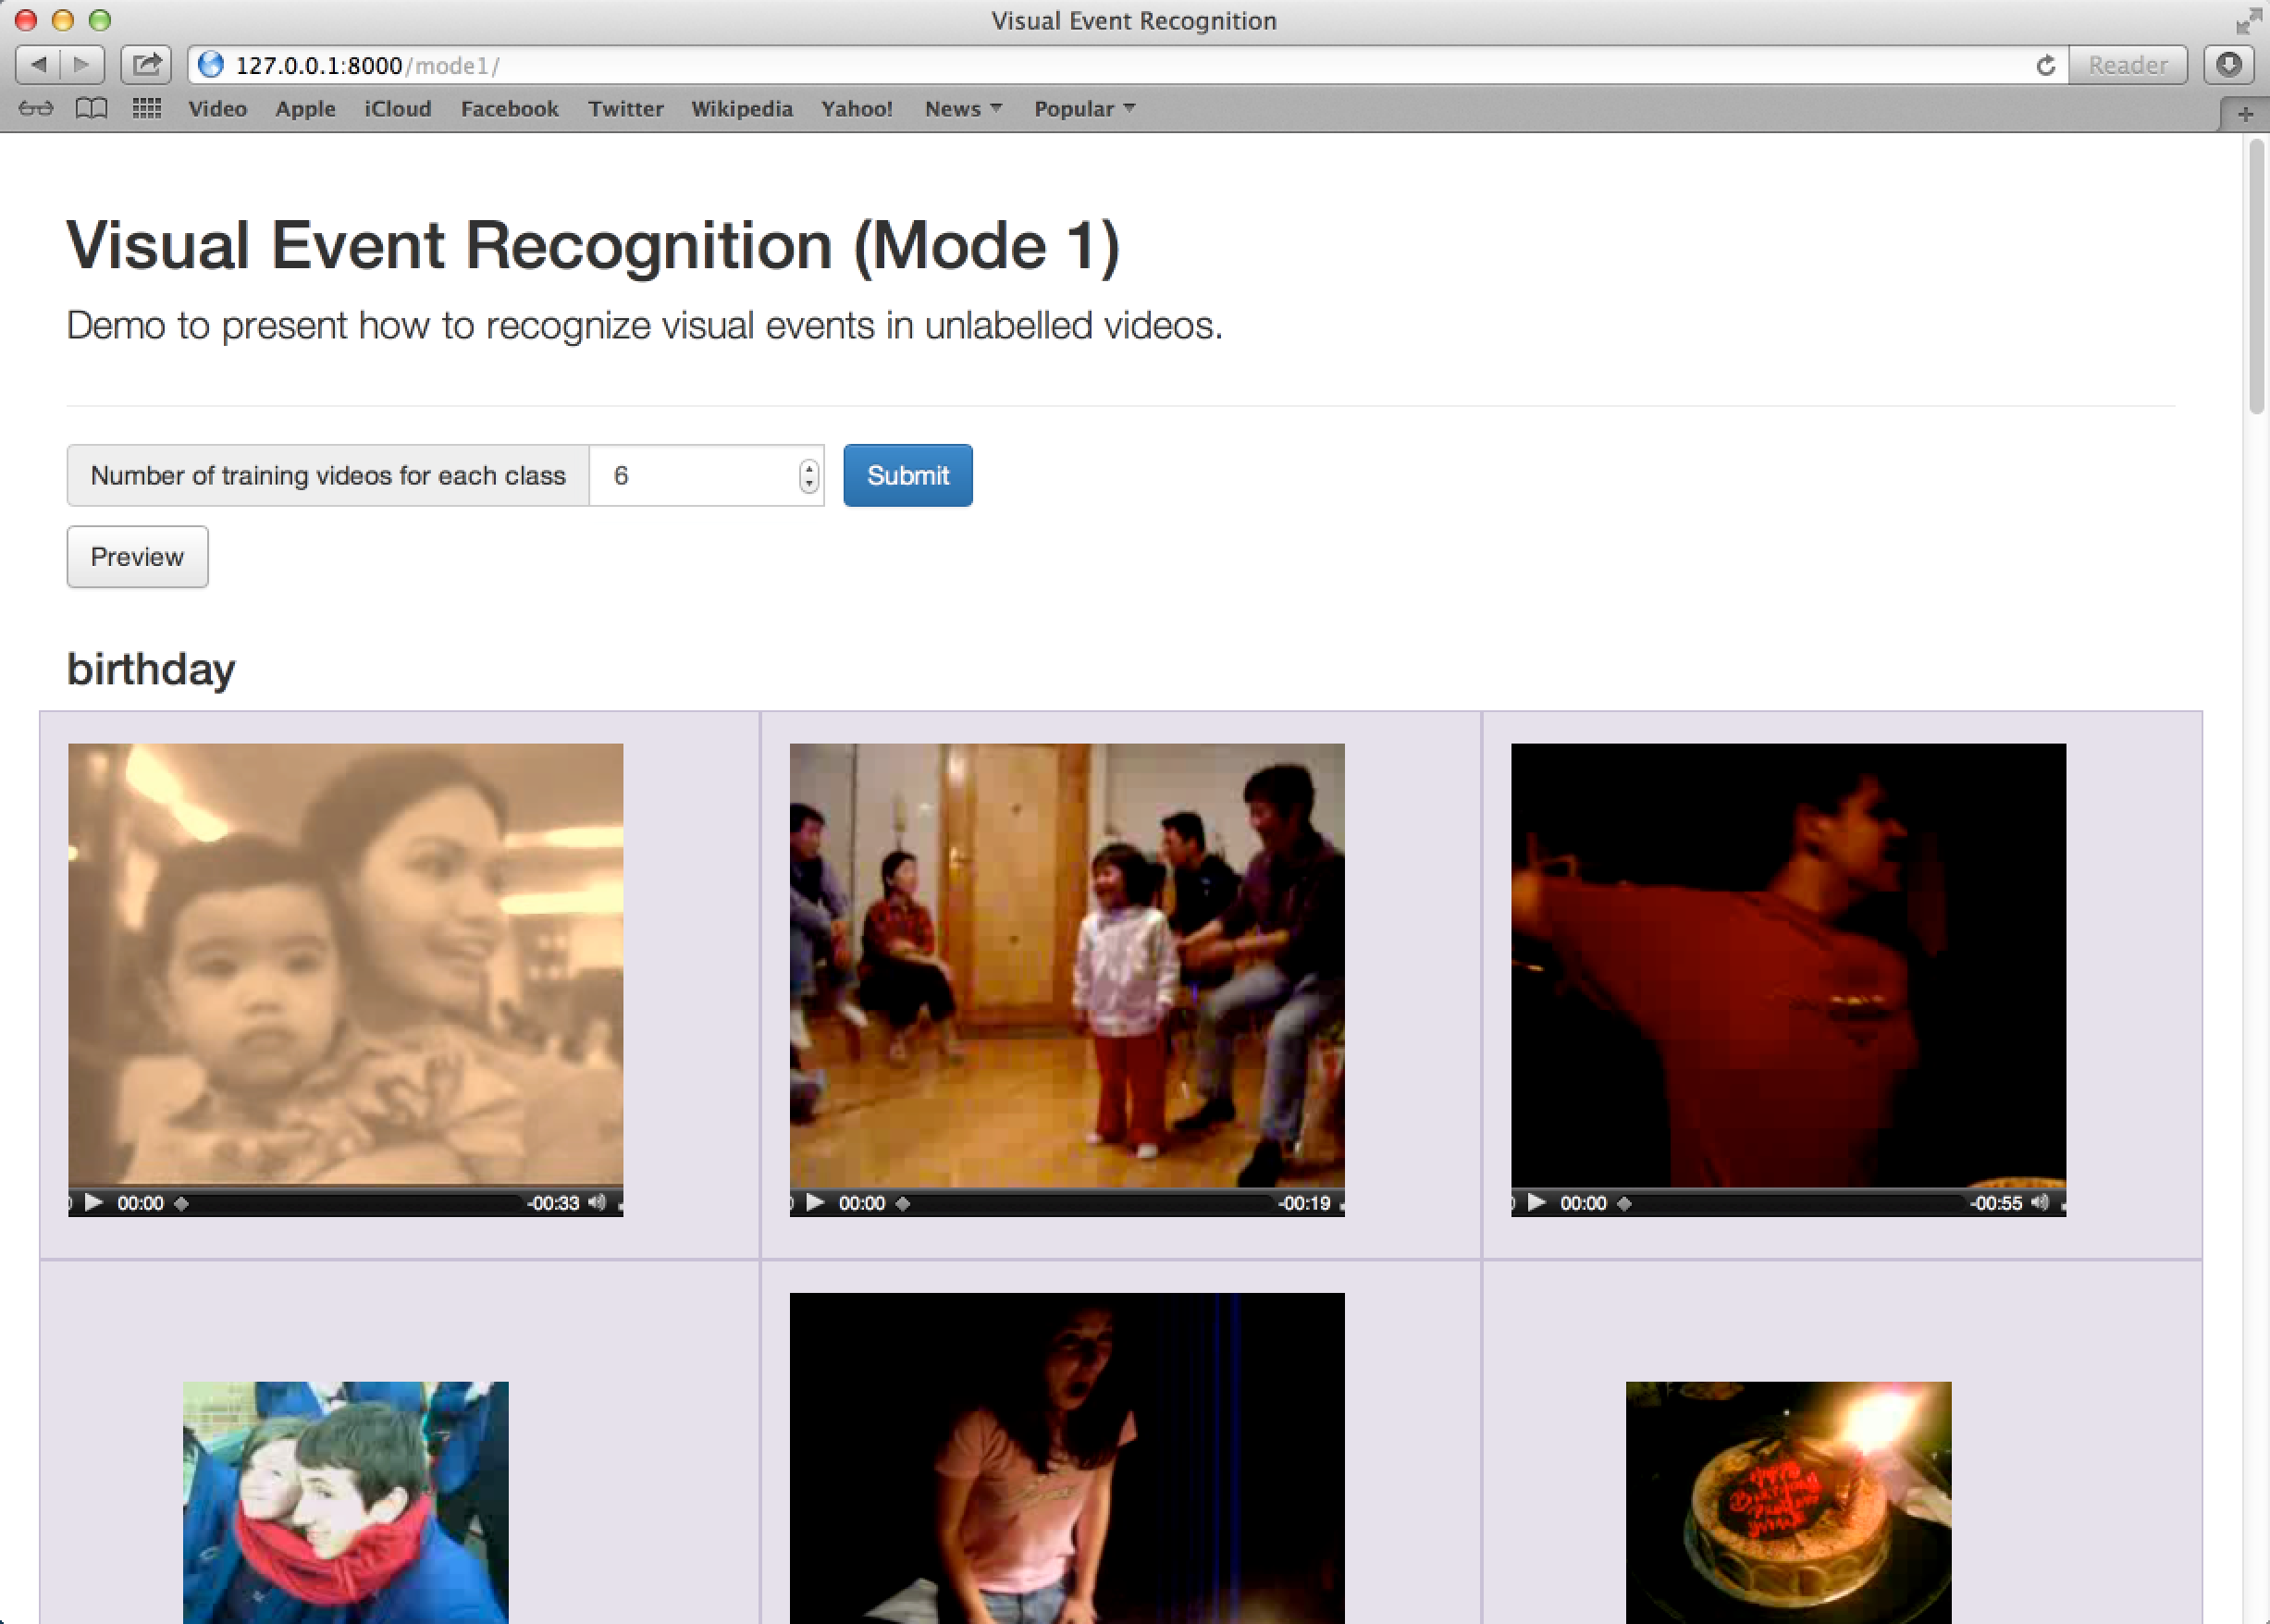
\includegraphics[scale=0.2]{./mode1.png}
\caption{Snapshot of mode 1. In mode 1, the distance matrix of Youtube videos is calculated offline. The user could randomly select the training data and testing data to check the recognition performance.}
\end{figure}

\begin{figure}[!ht]
\centering
	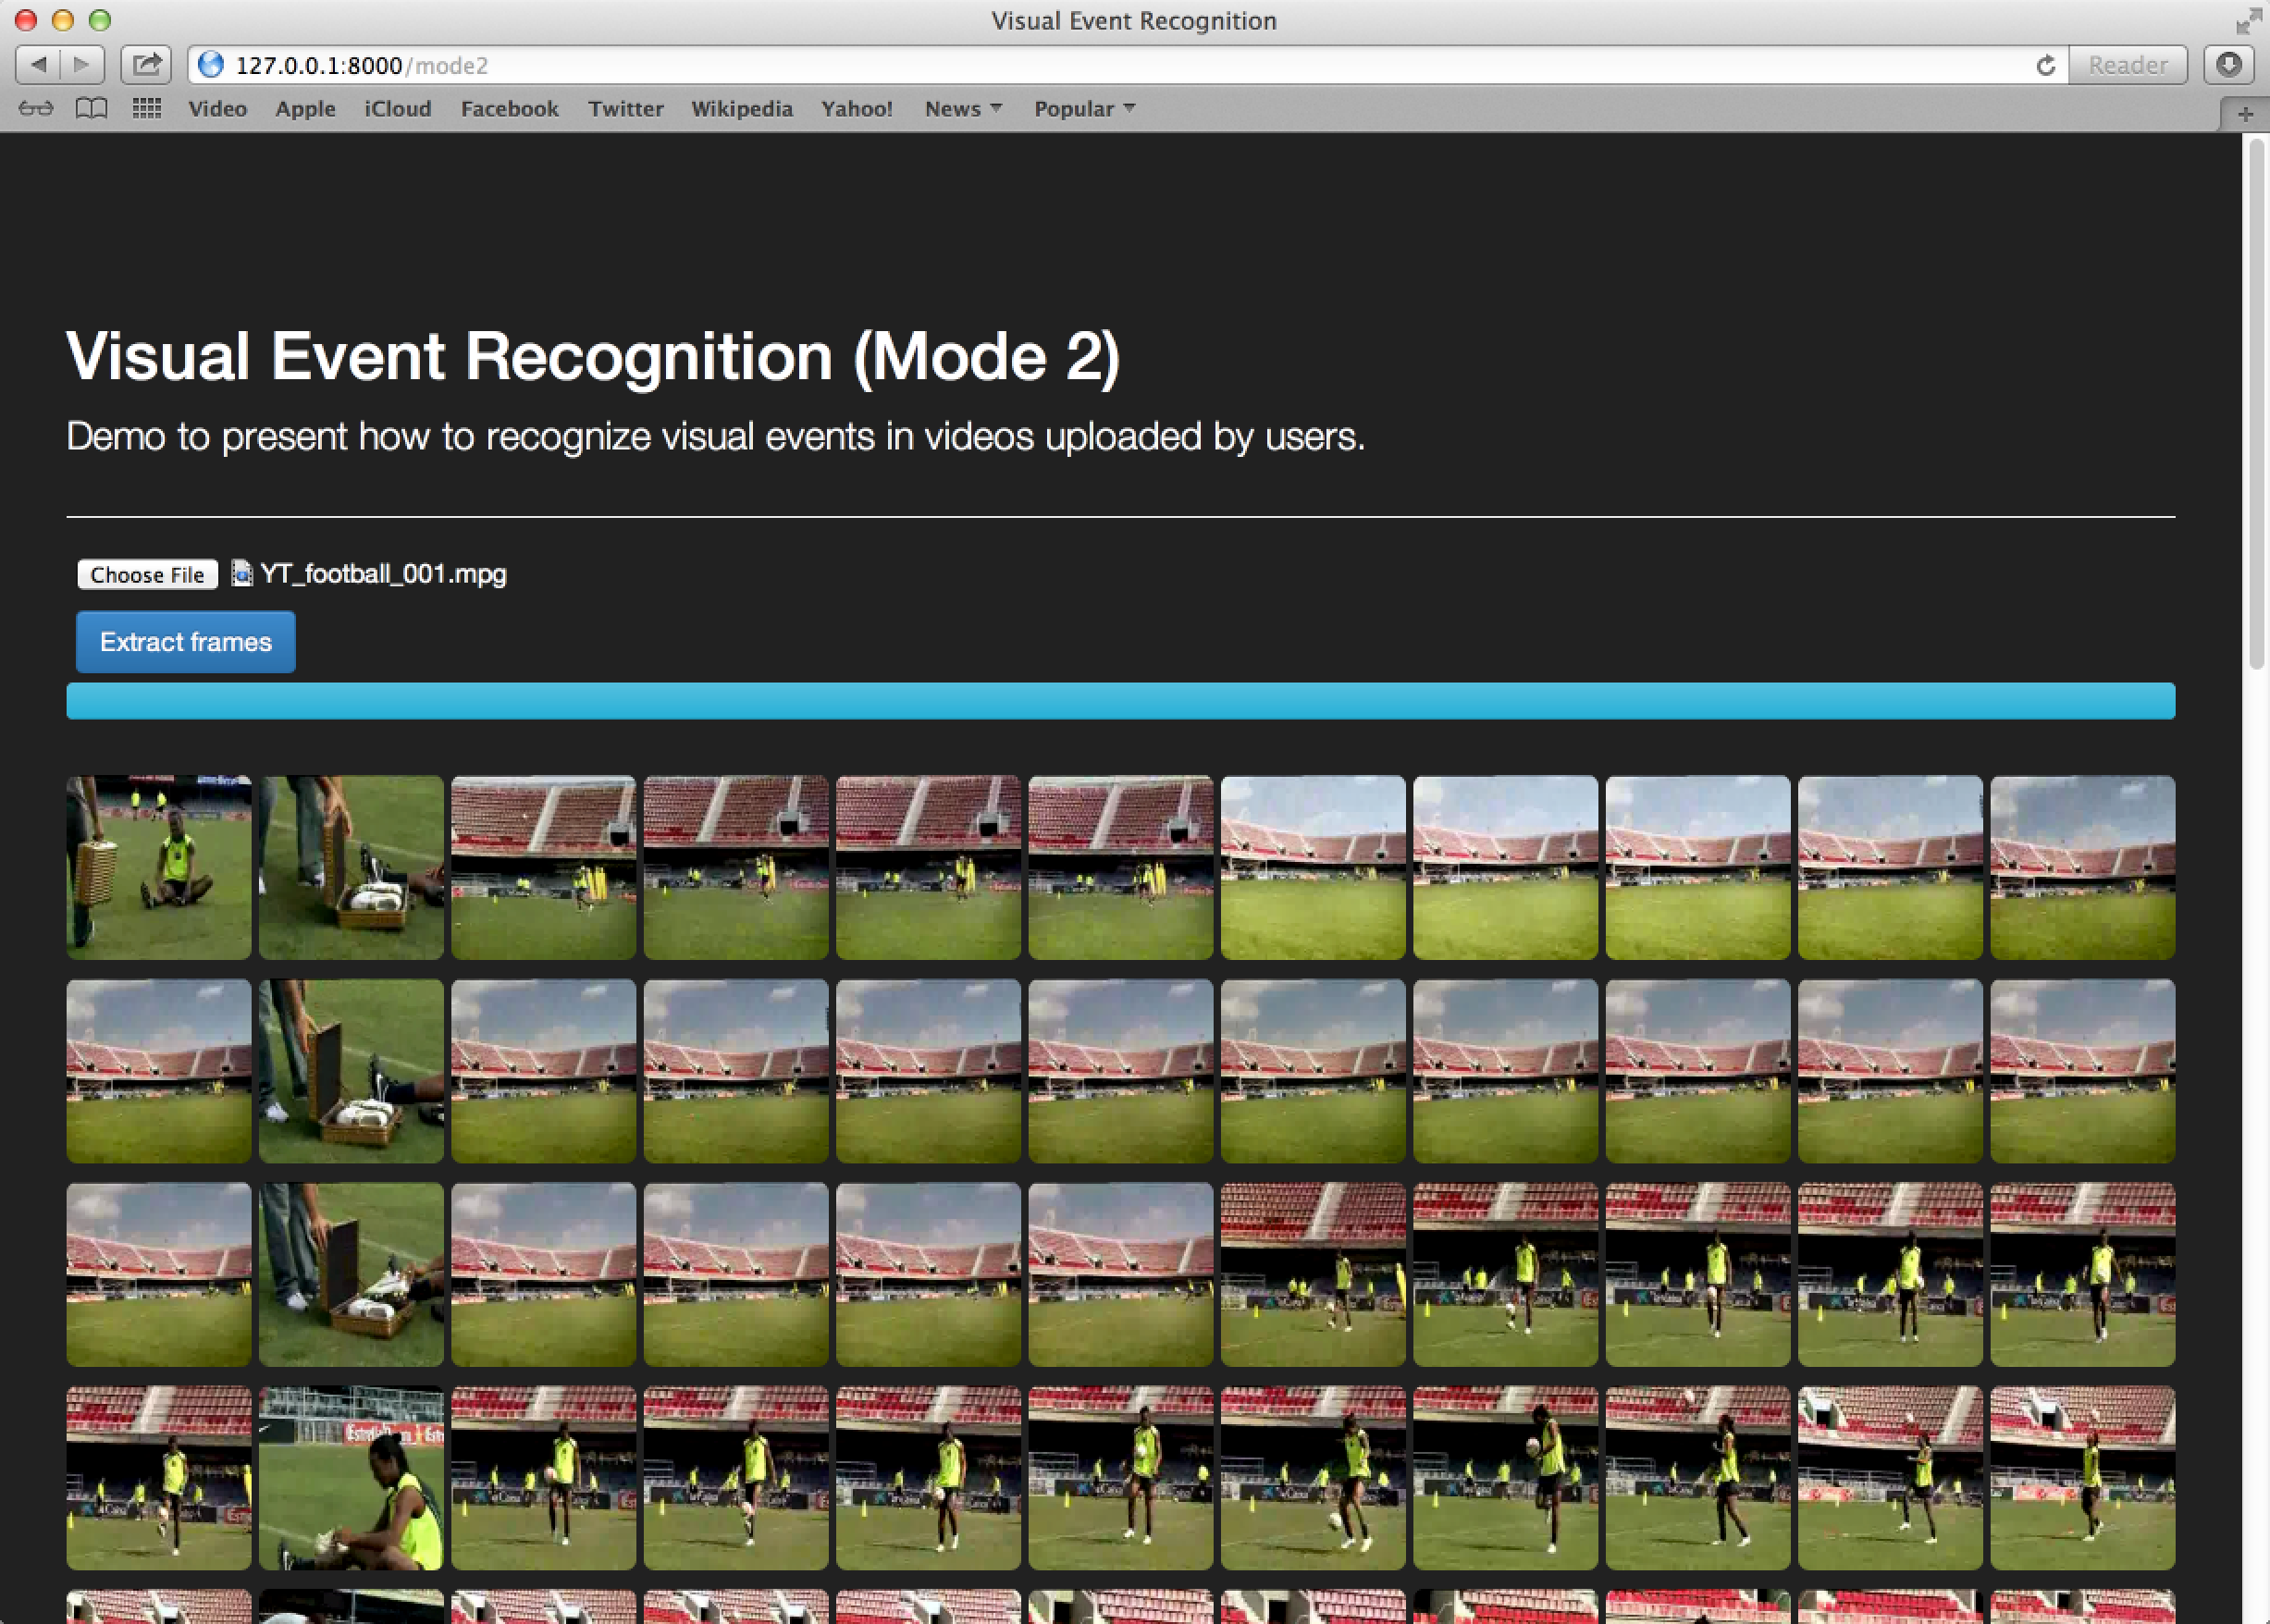
\includegraphics[scale = 0.2]{./mode2.png}
\caption{Snapshot of mode 2. In mode 2, the user could upload a new video and get the label of this video predicted by the underlying recognition system}
\end{figure}

\noindent There are two modes built for two different purposes as shown in Figure 15 and 16. Mode 1 enables the user to randomly select training and testing Youtube videos for recognition. The distance matrix of all Youtube videos used in recognition is calculated offline to save time. The second mode aims to present the user a whole process of recognizing videos. The user could upload a new video and check how this video is recognized from extracting frames, extracting features and building histograms all the way down to calculating distances with training videos and building a classifier for recognition. These two modes shall be able to present this project in a visualizable way. 